% Options for packages loaded elsewhere
\PassOptionsToPackage{unicode}{hyperref}
\PassOptionsToPackage{hyphens}{url}
%
\documentclass[
]{article}
\usepackage{amsmath,amssymb}
\usepackage{iftex}
\ifPDFTeX
  \usepackage[T1]{fontenc}
  \usepackage[utf8]{inputenc}
  \usepackage{textcomp} % provide euro and other symbols
\else % if luatex or xetex
  \usepackage{unicode-math} % this also loads fontspec
  \defaultfontfeatures{Scale=MatchLowercase}
  \defaultfontfeatures[\rmfamily]{Ligatures=TeX,Scale=1}
\fi
\usepackage{lmodern}
\ifPDFTeX\else
  % xetex/luatex font selection
  \setmainfont[]{Lato}
  \setmathfont[]{Lato Math}
\fi
% Use upquote if available, for straight quotes in verbatim environments
\IfFileExists{upquote.sty}{\usepackage{upquote}}{}
\IfFileExists{microtype.sty}{% use microtype if available
  \usepackage[]{microtype}
  \UseMicrotypeSet[protrusion]{basicmath} % disable protrusion for tt fonts
}{}
\makeatletter
\@ifundefined{KOMAClassName}{% if non-KOMA class
  \IfFileExists{parskip.sty}{%
    \usepackage{parskip}
  }{% else
    \setlength{\parindent}{0pt}
    \setlength{\parskip}{6pt plus 2pt minus 1pt}}
}{% if KOMA class
  \KOMAoptions{parskip=half}}
\makeatother
\usepackage{xcolor}
\usepackage[margin=1in]{geometry}
\usepackage{color}
\usepackage{fancyvrb}
\newcommand{\VerbBar}{|}
\newcommand{\VERB}{\Verb[commandchars=\\\{\}]}
\DefineVerbatimEnvironment{Highlighting}{Verbatim}{commandchars=\\\{\}}
% Add ',fontsize=\small' for more characters per line
\usepackage{framed}
\definecolor{shadecolor}{RGB}{248,248,248}
\newenvironment{Shaded}{\begin{snugshade}}{\end{snugshade}}
\newcommand{\AlertTok}[1]{\textcolor[rgb]{0.94,0.16,0.16}{#1}}
\newcommand{\AnnotationTok}[1]{\textcolor[rgb]{0.56,0.35,0.01}{\textbf{\textit{#1}}}}
\newcommand{\AttributeTok}[1]{\textcolor[rgb]{0.13,0.29,0.53}{#1}}
\newcommand{\BaseNTok}[1]{\textcolor[rgb]{0.00,0.00,0.81}{#1}}
\newcommand{\BuiltInTok}[1]{#1}
\newcommand{\CharTok}[1]{\textcolor[rgb]{0.31,0.60,0.02}{#1}}
\newcommand{\CommentTok}[1]{\textcolor[rgb]{0.56,0.35,0.01}{\textit{#1}}}
\newcommand{\CommentVarTok}[1]{\textcolor[rgb]{0.56,0.35,0.01}{\textbf{\textit{#1}}}}
\newcommand{\ConstantTok}[1]{\textcolor[rgb]{0.56,0.35,0.01}{#1}}
\newcommand{\ControlFlowTok}[1]{\textcolor[rgb]{0.13,0.29,0.53}{\textbf{#1}}}
\newcommand{\DataTypeTok}[1]{\textcolor[rgb]{0.13,0.29,0.53}{#1}}
\newcommand{\DecValTok}[1]{\textcolor[rgb]{0.00,0.00,0.81}{#1}}
\newcommand{\DocumentationTok}[1]{\textcolor[rgb]{0.56,0.35,0.01}{\textbf{\textit{#1}}}}
\newcommand{\ErrorTok}[1]{\textcolor[rgb]{0.64,0.00,0.00}{\textbf{#1}}}
\newcommand{\ExtensionTok}[1]{#1}
\newcommand{\FloatTok}[1]{\textcolor[rgb]{0.00,0.00,0.81}{#1}}
\newcommand{\FunctionTok}[1]{\textcolor[rgb]{0.13,0.29,0.53}{\textbf{#1}}}
\newcommand{\ImportTok}[1]{#1}
\newcommand{\InformationTok}[1]{\textcolor[rgb]{0.56,0.35,0.01}{\textbf{\textit{#1}}}}
\newcommand{\KeywordTok}[1]{\textcolor[rgb]{0.13,0.29,0.53}{\textbf{#1}}}
\newcommand{\NormalTok}[1]{#1}
\newcommand{\OperatorTok}[1]{\textcolor[rgb]{0.81,0.36,0.00}{\textbf{#1}}}
\newcommand{\OtherTok}[1]{\textcolor[rgb]{0.56,0.35,0.01}{#1}}
\newcommand{\PreprocessorTok}[1]{\textcolor[rgb]{0.56,0.35,0.01}{\textit{#1}}}
\newcommand{\RegionMarkerTok}[1]{#1}
\newcommand{\SpecialCharTok}[1]{\textcolor[rgb]{0.81,0.36,0.00}{\textbf{#1}}}
\newcommand{\SpecialStringTok}[1]{\textcolor[rgb]{0.31,0.60,0.02}{#1}}
\newcommand{\StringTok}[1]{\textcolor[rgb]{0.31,0.60,0.02}{#1}}
\newcommand{\VariableTok}[1]{\textcolor[rgb]{0.00,0.00,0.00}{#1}}
\newcommand{\VerbatimStringTok}[1]{\textcolor[rgb]{0.31,0.60,0.02}{#1}}
\newcommand{\WarningTok}[1]{\textcolor[rgb]{0.56,0.35,0.01}{\textbf{\textit{#1}}}}
\usepackage{graphicx}
\makeatletter
\def\maxwidth{\ifdim\Gin@nat@width>\linewidth\linewidth\else\Gin@nat@width\fi}
\def\maxheight{\ifdim\Gin@nat@height>\textheight\textheight\else\Gin@nat@height\fi}
\makeatother
% Scale images if necessary, so that they will not overflow the page
% margins by default, and it is still possible to overwrite the defaults
% using explicit options in \includegraphics[width, height, ...]{}
\setkeys{Gin}{width=\maxwidth,height=\maxheight,keepaspectratio}
% Set default figure placement to htbp
\makeatletter
\def\fps@figure{htbp}
\makeatother
\setlength{\emergencystretch}{3em} % prevent overfull lines
\providecommand{\tightlist}{%
  \setlength{\itemsep}{0pt}\setlength{\parskip}{0pt}}
\setcounter{secnumdepth}{-\maxdimen} % remove section numbering
\usepackage{booktabs}
\usepackage{longtable}
\usepackage{array}
\usepackage{multirow}
\usepackage{wrapfig}
\usepackage{float}
\usepackage{colortbl}
\usepackage{pdflscape}
\usepackage{tabu}
\usepackage{threeparttable}
\usepackage{threeparttablex}
\usepackage[normalem]{ulem}
\usepackage{makecell}
\usepackage{xcolor}
\ifLuaTeX
  \usepackage{selnolig}  % disable illegal ligatures
\fi
\IfFileExists{bookmark.sty}{\usepackage{bookmark}}{\usepackage{hyperref}}
\IfFileExists{xurl.sty}{\usepackage{xurl}}{} % add URL line breaks if available
\urlstyle{same}
\hypersetup{
  pdftitle={HW1-OLS\_Regression},
  hidelinks,
  pdfcreator={LaTeX via pandoc}}

\title{HW1-OLS\_Regression}
\author{}
\date{\vspace{-2.5em}2023-10-19}

\begin{document}
\maketitle

\[SSE = \sum(y_i - \hat{y_i})^2 = \sum[y_i - (\beta_0 + \]

\hypertarget{introduction}{%
\section{Introduction}\label{introduction}}

\hypertarget{methods}{%
\section{Methods}\label{methods}}

\hypertarget{data-cleaning}{%
\subsection{Data Cleaning}\label{data-cleaning}}

The data set used in our analysis contains information from the 2000 US
Census for Philadelphia, with neighborhood characteristic variables
included for 1,720 block groups. Our analysis incorporates the following
variables:

\begin{itemize}
\tightlist
\item
  POLY\_ID: Census Block Group ID
\item
  MEDHVAL: Median value of all owner occupied housing units
\item
  PCBACHMORE: Proportion of residents in Block Group with at least a
  bachelor's degree
\item
  PCTVACANT: Proportion of housing units that are vacant
\item
  PCTSINGLES: Percent of housing units that are detached single family
  houses
\item
  NBELPOV100: Number of households with incomes below 100\% poverty
  level (i.e., number of households living in poverty)
\item
  MEDHHINC: Median household income
\end{itemize}

The original data set had 1,816 block groups and was cleaned using the
following methods, which reduced to the total number of observations to
1,720:

\begin{itemize}
\tightlist
\item
  Block groups where population \textless{} 40
\item
  Block groups where there are no housing units
\item
  Block groups where the median house value is lower than \$10,000
\item
  One North Philadelphia block group which had a very high median house
  value (over \$800,000) and a very low median household income (less
  than \$8,000)
\end{itemize}

In this analysis, we will examine the relationships between our
dependent variable, MEDHVAL, and the predictors PCBACHMORE, NBELPOV100,
PCTVACANT, and PCTSINGLES.

\hypertarget{exploratory-data-analysis}{%
\subsection{Exploratory Data Analysis}\label{exploratory-data-analysis}}

We will examine the summary statistics and distributions of the data
set's variables, including the mean and standard deviation of our
dependent variable and predictor variables.

As part of our exploratory data analysis, we will examine the Pearson
correlations between the predictors. A Pearson correlation, denoted by
``r'', is a standardized measurement of the strength and direction of
the linear relationship between two variables. The correlation between
two variables is calculated using the following equation:

\[r=\frac{1}{n-1}\sum_{i=1}^{n}\left(\frac{x_i-x ̅}{s_x}\right)\left(\frac{y_i-y ̅}{s_x}\right)\]

The Pearson correlation value ranges between -1 to 1, with no units of
measurement attached, and the observed variables are interchangeable
between the x axis and y axis. A value of -1 represents a perfect
negative linear relationship and a value of 1 represents a perfect
positive linear relationship - in either case, points on a graph would
appear in a straight line with either a negative or positive slope,
respectively.

A Pearson correlation value of 0 indicates that there is no linear
relationship between two variables. However, a different type of
relationship can exist, such as an exponential or quadratic
relationship, that the Pearson correlation does not measure.

\hypertarget{multiple-regression-analysis}{%
\subsection{Multiple Regression
Analysis}\label{multiple-regression-analysis}}

\hypertarget{additional-analyses}{%
\subsection{Additional Analyses}\label{additional-analyses}}

\hypertarget{software}{%
\subsection{Software}\label{software}}

This report used the open source software R to conduct statistical
analyses.

\hypertarget{results}{%
\section{Results}\label{results}}

\hypertarget{exploratory-results}{%
\subsection{Exploratory Results}\label{exploratory-results}}

\begin{Shaded}
\begin{Highlighting}[]
\NormalTok{data }\OtherTok{\textless{}{-}} \FunctionTok{read.csv}\NormalTok{(}\StringTok{"Data/RegressionData.csv"}\NormalTok{)}
\end{Highlighting}
\end{Shaded}

\begin{Shaded}
\begin{Highlighting}[]
\NormalTok{summary\_stats\_mean }\OtherTok{\textless{}{-}}\NormalTok{ data }\SpecialCharTok{\%\textgreater{}\%}
  \FunctionTok{summarise}\NormalTok{(}\AttributeTok{HEDVAL =} \FunctionTok{mean}\NormalTok{(MEDHVAL),}
            \AttributeTok{PCTBACHMOR =} \FunctionTok{mean}\NormalTok{(PCTBACHMOR),}
            \AttributeTok{NBELPOV100 =} \FunctionTok{mean}\NormalTok{(NBELPOV100),}
            \AttributeTok{PCTVACANT =} \FunctionTok{mean}\NormalTok{(PCTVACANT),}
            \AttributeTok{PCTSINGLE =} \FunctionTok{mean}\NormalTok{(PCTSINGLES)) }\SpecialCharTok{\%\textgreater{}\%}
  \FunctionTok{gather}\NormalTok{(}\AttributeTok{key =} \StringTok{"variable"}\NormalTok{, }\AttributeTok{value =} \StringTok{"mean"}\NormalTok{)}
            
\NormalTok{summary\_stats\_sd }\OtherTok{\textless{}{-}}\NormalTok{ data }\SpecialCharTok{\%\textgreater{}\%}
  \FunctionTok{summarise}\NormalTok{(}\AttributeTok{HEDVAL =} \FunctionTok{sd}\NormalTok{(MEDHVAL),}
            \AttributeTok{PCTBACHMOR =} \FunctionTok{sd}\NormalTok{(PCTBACHMOR),}
            \AttributeTok{NBELPOV100 =} \FunctionTok{sd}\NormalTok{(NBELPOV100),}
            \AttributeTok{PCTVACANT =} \FunctionTok{sd}\NormalTok{(PCTVACANT),}
            \AttributeTok{PCTSINGLE =} \FunctionTok{sd}\NormalTok{(PCTSINGLES)) }\SpecialCharTok{\%\textgreater{}\%}
  \FunctionTok{gather}\NormalTok{(}\AttributeTok{key =} \StringTok{"variable"}\NormalTok{, }\AttributeTok{value =} \StringTok{"sd"}\NormalTok{) }\SpecialCharTok{\%\textgreater{}\%}
  \FunctionTok{mutate}\NormalTok{(}\AttributeTok{row\_names =} \FunctionTok{c}\NormalTok{(}\StringTok{\textquotesingle{}Median Houme Value of all occupied housing units\textquotesingle{}}\NormalTok{,}\StringTok{\textquotesingle{}\% of Individuals with Bachelor Degrees or Higher\textquotesingle{}}\NormalTok{,}\StringTok{\textquotesingle{}\# Households Living in Poverty\textquotesingle{}}\NormalTok{,}\StringTok{\textquotesingle{}\% of Vacant Houses\textquotesingle{}}\NormalTok{,}\StringTok{\textquotesingle{}\% of Single House Units\textquotesingle{}}\NormalTok{)) }

\FunctionTok{left\_join}\NormalTok{(summary\_stats\_mean, summary\_stats\_sd, }\AttributeTok{by=}\StringTok{\textquotesingle{}variable\textquotesingle{}}\NormalTok{) }\SpecialCharTok{\%\textgreater{}\%}
\NormalTok{  dplyr}\SpecialCharTok{::}\FunctionTok{select}\NormalTok{(}\StringTok{\textquotesingle{}row\_names\textquotesingle{}}\NormalTok{,}\StringTok{\textquotesingle{}mean\textquotesingle{}}\NormalTok{,}\StringTok{\textquotesingle{}sd\textquotesingle{}}\NormalTok{) }\SpecialCharTok{\%\textgreater{}\%}
  \FunctionTok{kbl}\NormalTok{(}\AttributeTok{col.names =} \FunctionTok{c}\NormalTok{(}\StringTok{\textquotesingle{}Variable\textquotesingle{}}\NormalTok{,}\StringTok{\textquotesingle{}Mean\textquotesingle{}}\NormalTok{,}\StringTok{\textquotesingle{}Standard Deviation\textquotesingle{}}\NormalTok{)) }\SpecialCharTok{\%\textgreater{}\%}
  \FunctionTok{kable\_classic}\NormalTok{()}
\end{Highlighting}
\end{Shaded}

\begin{table}
\centering
\begin{tabular}[t]{l|r|r}
\hline
Variable & Mean & Standard Deviation\\
\hline
Median Houme Value of all occupied housing units & 66287.733139 & 60006.075990\\
\hline
\% of Individuals with Bachelor Degrees or Higher & 16.081372 & 17.769558\\
\hline
\# Households Living in Poverty & 189.770930 & 164.318480\\
\hline
\% of Vacant Houses & 11.288529 & 9.628472\\
\hline
\% of Single House Units & 9.226473 & 13.249250\\
\hline
\end{tabular}
\end{table}

\hypertarget{quick-code-that-checks-which-variables-have-0-values-for-logarithmic-transformation}{%
\section{quick code that checks which variables have 0 values for
logarithmic
transformation}\label{quick-code-that-checks-which-variables-have-0-values-for-logarithmic-transformation}}

\begin{Shaded}
\begin{Highlighting}[]
\NormalTok{zero\_columns }\OtherTok{\textless{}{-}} \FunctionTok{apply}\NormalTok{(data, }\DecValTok{2}\NormalTok{, }\ControlFlowTok{function}\NormalTok{(col) }\FunctionTok{any}\NormalTok{(col }\SpecialCharTok{==} \DecValTok{0}\NormalTok{)) }

\NormalTok{variables\_with\_zero\_values }\OtherTok{\textless{}{-}} \FunctionTok{names}\NormalTok{(zero\_columns[zero\_columns])}

\FunctionTok{cat}\NormalTok{(}\StringTok{"Columns with 0 values:"}\NormalTok{, }\FunctionTok{paste}\NormalTok{(variables\_with\_zero\_values, }\AttributeTok{collapse =} \StringTok{", "}\NormalTok{))}
\end{Highlighting}
\end{Shaded}

\begin{verbatim}
## Columns with 0 values: PCTBACHMOR, PCTVACANT, PCTSINGLES, NBELPOV100
\end{verbatim}

\begin{Shaded}
\begin{Highlighting}[]
\NormalTok{data}\SpecialCharTok{$}\NormalTok{LNMEDHVAL }\OtherTok{\textless{}{-}} \FunctionTok{log}\NormalTok{(data}\SpecialCharTok{$}\NormalTok{MEDHVAL)}
\NormalTok{data}\SpecialCharTok{$}\NormalTok{LNPCTBACHMOR }\OtherTok{\textless{}{-}} \FunctionTok{log}\NormalTok{(}\DecValTok{1} \SpecialCharTok{+}\NormalTok{ data}\SpecialCharTok{$}\NormalTok{PCTBACHMOR)}
\NormalTok{data}\SpecialCharTok{$}\NormalTok{LNBELPOV100 }\OtherTok{\textless{}{-}} \FunctionTok{log}\NormalTok{(}\DecValTok{1} \SpecialCharTok{+}\NormalTok{ data}\SpecialCharTok{$}\NormalTok{NBELPOV100) }\CommentTok{\#Rename and add N to match original name?}
\NormalTok{data}\SpecialCharTok{$}\NormalTok{LNPCTVACANT }\OtherTok{\textless{}{-}} \FunctionTok{log}\NormalTok{(}\DecValTok{1} \SpecialCharTok{+}\NormalTok{ data}\SpecialCharTok{$}\NormalTok{PCTVACANT)}
\NormalTok{data}\SpecialCharTok{$}\NormalTok{LNPCTSINGLES }\OtherTok{\textless{}{-}} \FunctionTok{log}\NormalTok{(}\DecValTok{1} \SpecialCharTok{+}\NormalTok{ data}\SpecialCharTok{$}\NormalTok{PCTSINGLES)}
\end{Highlighting}
\end{Shaded}

\begin{Shaded}
\begin{Highlighting}[]
\FunctionTok{par}\NormalTok{(}\AttributeTok{mfrow=}\FunctionTok{c}\NormalTok{(}\DecValTok{1}\NormalTok{,}\DecValTok{2}\NormalTok{))}
\FunctionTok{hist}\NormalTok{(data}\SpecialCharTok{$}\NormalTok{MEDHVAL,}\AttributeTok{breaks=}\DecValTok{100}\NormalTok{)}
\FunctionTok{hist}\NormalTok{(data}\SpecialCharTok{$}\NormalTok{LNMEDHVAL,}\AttributeTok{breaks=}\DecValTok{100}\NormalTok{)}
\end{Highlighting}
\end{Shaded}


\includegraphics{HW1-Regression_files/figure-latex/hist_MEDHVAL-1.pdf}

\begin{Shaded}
\begin{Highlighting}[]
\FunctionTok{par}\NormalTok{(}\AttributeTok{mfrow=}\FunctionTok{c}\NormalTok{(}\DecValTok{1}\NormalTok{,}\DecValTok{2}\NormalTok{))}
\FunctionTok{hist}\NormalTok{(data}\SpecialCharTok{$}\NormalTok{PCTBACHMOR,}\AttributeTok{breaks=}\DecValTok{100}\NormalTok{)}
\FunctionTok{hist}\NormalTok{(data}\SpecialCharTok{$}\NormalTok{LNPCTBACHMOR,}\AttributeTok{breaks=}\DecValTok{100}\NormalTok{)}
\end{Highlighting}
\end{Shaded}

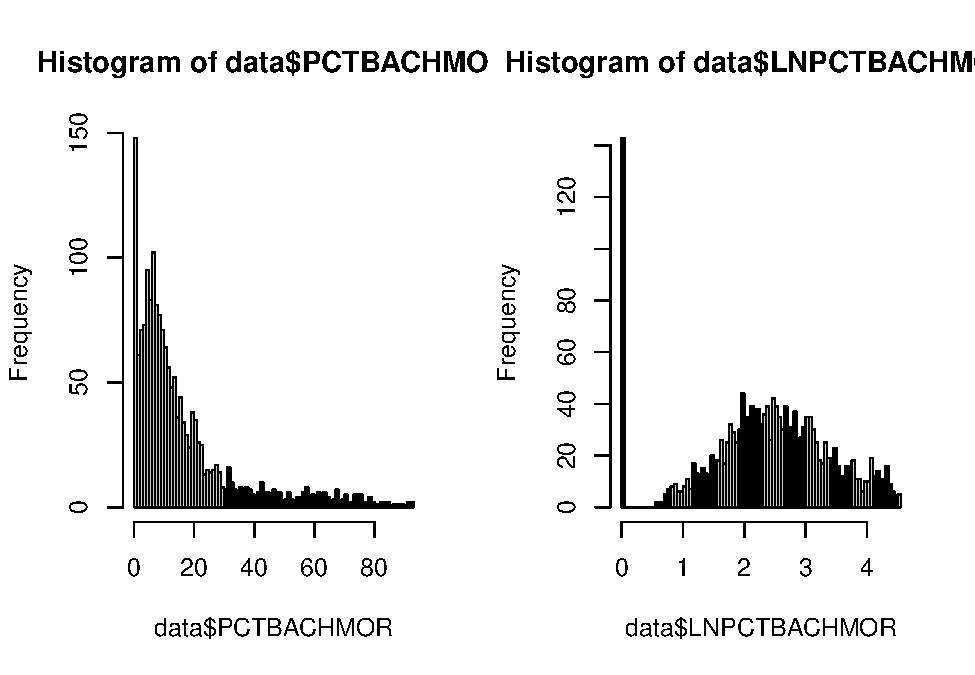
\includegraphics{HW1-Regression_files/figure-latex/hist_PCTBACHMOR-1.pdf}

\begin{Shaded}
\begin{Highlighting}[]
\FunctionTok{par}\NormalTok{(}\AttributeTok{mfrow=}\FunctionTok{c}\NormalTok{(}\DecValTok{1}\NormalTok{,}\DecValTok{2}\NormalTok{))}
\FunctionTok{hist}\NormalTok{(data}\SpecialCharTok{$}\NormalTok{NBELPOV100,}\AttributeTok{breaks=}\DecValTok{100}\NormalTok{)}
\FunctionTok{hist}\NormalTok{(data}\SpecialCharTok{$}\NormalTok{LNBELPOV100,}\AttributeTok{breaks=}\DecValTok{100}\NormalTok{)}
\end{Highlighting}
\end{Shaded}

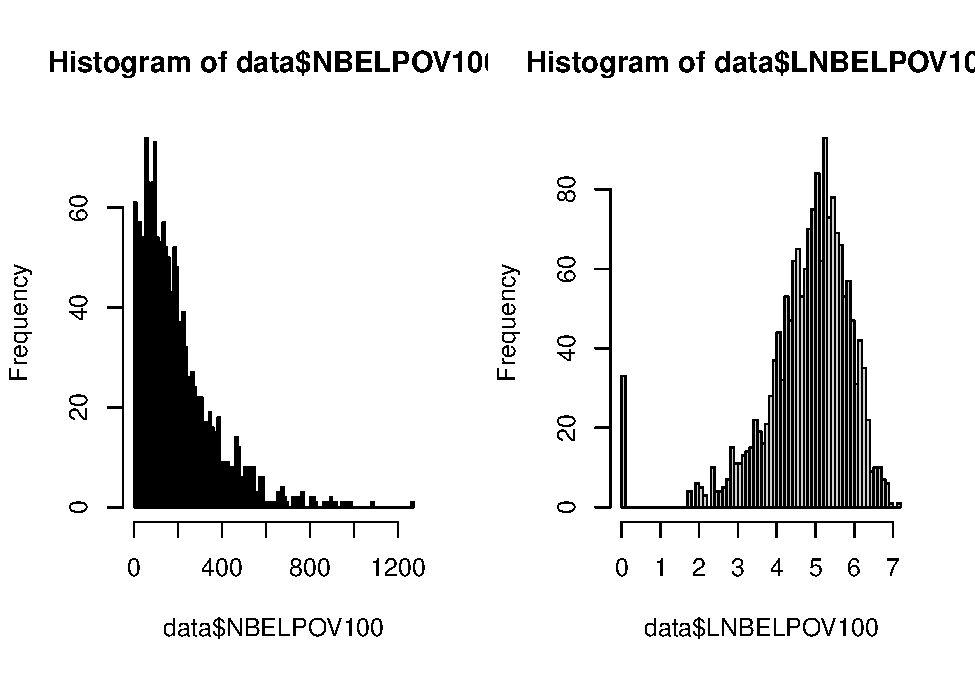
\includegraphics{HW1-Regression_files/figure-latex/hist_NBELPOV100-1.pdf}

\begin{Shaded}
\begin{Highlighting}[]
\FunctionTok{par}\NormalTok{(}\AttributeTok{mfrow=}\FunctionTok{c}\NormalTok{(}\DecValTok{1}\NormalTok{,}\DecValTok{2}\NormalTok{))}
\FunctionTok{hist}\NormalTok{(data}\SpecialCharTok{$}\NormalTok{PCTVACANT,}\AttributeTok{breaks=}\DecValTok{100}\NormalTok{)}
\FunctionTok{hist}\NormalTok{(data}\SpecialCharTok{$}\NormalTok{LNPCTVACANT,}\AttributeTok{breaks=}\DecValTok{100}\NormalTok{)}
\end{Highlighting}
\end{Shaded}

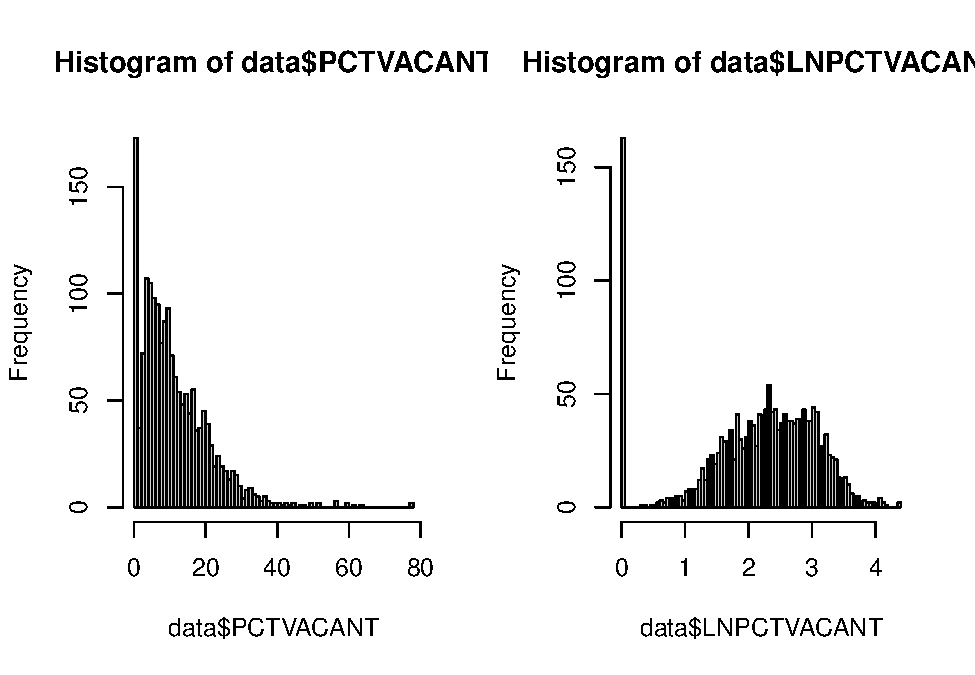
\includegraphics{HW1-Regression_files/figure-latex/hist_PCTVACANT-1.pdf}

\begin{Shaded}
\begin{Highlighting}[]
\FunctionTok{par}\NormalTok{(}\AttributeTok{mfrow=}\FunctionTok{c}\NormalTok{(}\DecValTok{1}\NormalTok{,}\DecValTok{2}\NormalTok{))}
\FunctionTok{hist}\NormalTok{(data}\SpecialCharTok{$}\NormalTok{PCTSINGLES,}\AttributeTok{breaks=}\DecValTok{100}\NormalTok{)}
\FunctionTok{hist}\NormalTok{(data}\SpecialCharTok{$}\NormalTok{LNPCTSINGLES,}\AttributeTok{breaks=}\DecValTok{100}\NormalTok{)}
\end{Highlighting}
\end{Shaded}

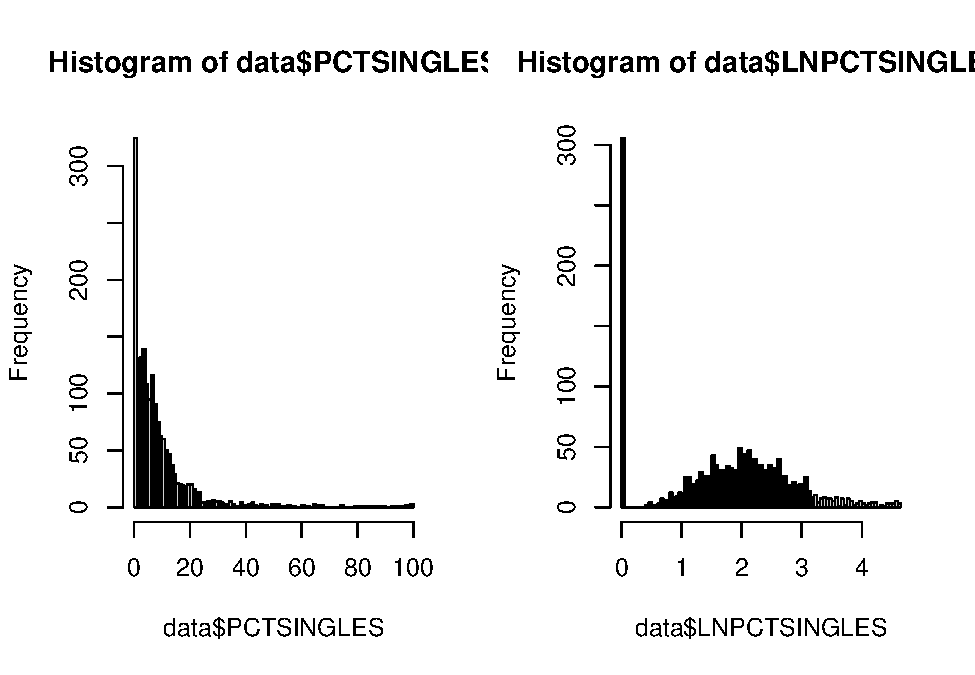
\includegraphics{HW1-Regression_files/figure-latex/hist_PCTSINGLES-1.pdf}

\begin{Shaded}
\begin{Highlighting}[]
\CommentTok{\# Change design}
\NormalTok{map }\OtherTok{\textless{}{-}} \FunctionTok{st\_read}\NormalTok{(}\StringTok{"Data/RegressionData.shp"}\NormalTok{)}
\end{Highlighting}
\end{Shaded}

\begin{verbatim}
## Reading layer `RegressionData' from data source 
##   `D:\Penn\Stats\MUSA500-HW1\Data\RegressionData.shp' using driver `ESRI Shapefile'
## Simple feature collection with 1720 features and 13 fields
## Geometry type: POLYGON
## Dimension:     XY
## Bounding box:  xmin: 2660605 ymin: 207610.6 xmax: 2750171 ymax: 304858.8
## CRS:           NA
\end{verbatim}

\begin{Shaded}
\begin{Highlighting}[]
\FunctionTok{ggplot}\NormalTok{() }\SpecialCharTok{+}
  \FunctionTok{geom\_sf}\NormalTok{(}\AttributeTok{data =}\NormalTok{ map, }\FunctionTok{aes}\NormalTok{(}\AttributeTok{fill =}\NormalTok{ LNMEDHVAL), }\AttributeTok{color =} \ConstantTok{NA}\NormalTok{) }\SpecialCharTok{+}
  \FunctionTok{scale\_fill\_gradient}\NormalTok{(}\AttributeTok{low =} \StringTok{"white"}\NormalTok{,}\AttributeTok{high =} \StringTok{"darkseagreen4"}\NormalTok{) }\SpecialCharTok{+}
  \FunctionTok{labs}\NormalTok{(}\AttributeTok{title =} \StringTok{"Log Median Home Value"}\NormalTok{) }\SpecialCharTok{+}
  \FunctionTok{theme\_dark}\NormalTok{() }\SpecialCharTok{+}
  \FunctionTok{theme}\NormalTok{( }
    \AttributeTok{panel.grid.major =} \FunctionTok{element\_blank}\NormalTok{(),}
    \AttributeTok{panel.grid.minor =} \FunctionTok{element\_blank}\NormalTok{(),}
    \AttributeTok{axis.ticks =} \FunctionTok{element\_blank}\NormalTok{(),}
    \AttributeTok{axis.text =} \FunctionTok{element\_blank}\NormalTok{()}
\NormalTok{    )}
\end{Highlighting}
\end{Shaded}

\includegraphics{HW1-Regression_files/figure-latex/LNMEDHVAL map-1.pdf}

\begin{Shaded}
\begin{Highlighting}[]
\CommentTok{\# Change designs}
\NormalTok{pctvacant\_map }\OtherTok{\textless{}{-}} \FunctionTok{ggplot}\NormalTok{() }\SpecialCharTok{+}
  \FunctionTok{geom\_sf}\NormalTok{(}\AttributeTok{data =}\NormalTok{ map, }\FunctionTok{aes}\NormalTok{(}\AttributeTok{fill =}\NormalTok{ PCTVACANT), }\AttributeTok{color =} \ConstantTok{NA}\NormalTok{) }\SpecialCharTok{+}
  \FunctionTok{scale\_fill\_gradient}\NormalTok{(}\AttributeTok{low =} \StringTok{"white"}\NormalTok{,}\AttributeTok{high =} \StringTok{"darkblue"}\NormalTok{) }\SpecialCharTok{+}
  \FunctionTok{labs}\NormalTok{(}\AttributeTok{title =} \StringTok{"Vacant"}\NormalTok{,}
       \AttributeTok{fill =} \StringTok{"\%"}\NormalTok{)}\SpecialCharTok{+}
  \FunctionTok{theme\_dark}\NormalTok{() }\SpecialCharTok{+}
  \FunctionTok{theme}\NormalTok{( }
    \AttributeTok{panel.grid.major =} \FunctionTok{element\_blank}\NormalTok{(),}
    \AttributeTok{panel.grid.minor =} \FunctionTok{element\_blank}\NormalTok{(),}
    \AttributeTok{axis.ticks =} \FunctionTok{element\_blank}\NormalTok{(),}
    \AttributeTok{axis.text =} \FunctionTok{element\_blank}\NormalTok{()}
\NormalTok{    )}

\NormalTok{pctsingles\_map }\OtherTok{\textless{}{-}} \FunctionTok{ggplot}\NormalTok{() }\SpecialCharTok{+}
  \FunctionTok{geom\_sf}\NormalTok{(}\AttributeTok{data =}\NormalTok{ map, }\FunctionTok{aes}\NormalTok{(}\AttributeTok{fill =}\NormalTok{ PCTSINGLES), }\AttributeTok{color =} \ConstantTok{NA}\NormalTok{) }\SpecialCharTok{+}
  \FunctionTok{scale\_fill\_gradient}\NormalTok{(}\AttributeTok{low =} \StringTok{"white"}\NormalTok{,}\AttributeTok{high =} \StringTok{"darkorchid4"}\NormalTok{) }\SpecialCharTok{+}
  \FunctionTok{labs}\NormalTok{(}\AttributeTok{title =} \StringTok{"Singles"}\NormalTok{,}
       \AttributeTok{fill =} \StringTok{"\%"}\NormalTok{)}\SpecialCharTok{+}
  \FunctionTok{theme\_dark}\NormalTok{() }\SpecialCharTok{+}
  \FunctionTok{theme}\NormalTok{( }
    \AttributeTok{panel.grid.major =} \FunctionTok{element\_blank}\NormalTok{(),}
    \AttributeTok{panel.grid.minor =} \FunctionTok{element\_blank}\NormalTok{(),}
    \AttributeTok{axis.ticks =} \FunctionTok{element\_blank}\NormalTok{(),}
    \AttributeTok{axis.text =} \FunctionTok{element\_blank}\NormalTok{()}
\NormalTok{    )}

\NormalTok{pctbachmor\_map }\OtherTok{\textless{}{-}} \FunctionTok{ggplot}\NormalTok{() }\SpecialCharTok{+}
  \FunctionTok{geom\_sf}\NormalTok{(}\AttributeTok{data =}\NormalTok{ map, }\FunctionTok{aes}\NormalTok{(}\AttributeTok{fill =}\NormalTok{ PCTBACHMOR), }\AttributeTok{color =} \ConstantTok{NA}\NormalTok{) }\SpecialCharTok{+}
  \FunctionTok{scale\_fill\_gradient}\NormalTok{(}\AttributeTok{low =} \StringTok{"white"}\NormalTok{,}\AttributeTok{high =} \StringTok{"darkorange"}\NormalTok{) }\SpecialCharTok{+}
  \FunctionTok{labs}\NormalTok{(}\AttributeTok{title =} \StringTok{"Bachelor\textquotesingle{}s or More"}\NormalTok{,}
       \AttributeTok{fill =} \StringTok{"\%"}\NormalTok{)}\SpecialCharTok{+}
  \FunctionTok{theme\_dark}\NormalTok{() }\SpecialCharTok{+}
  \FunctionTok{theme}\NormalTok{( }
    \AttributeTok{panel.grid.major =} \FunctionTok{element\_blank}\NormalTok{(),}
    \AttributeTok{panel.grid.minor =} \FunctionTok{element\_blank}\NormalTok{(),}
    \AttributeTok{axis.ticks =} \FunctionTok{element\_blank}\NormalTok{(),}
    \AttributeTok{axis.text =} \FunctionTok{element\_blank}\NormalTok{()}
\NormalTok{    )}

\NormalTok{lnnbelpov100\_map }\OtherTok{\textless{}{-}} \FunctionTok{ggplot}\NormalTok{() }\SpecialCharTok{+}
  \FunctionTok{geom\_sf}\NormalTok{(}\AttributeTok{data =}\NormalTok{ map, }\FunctionTok{aes}\NormalTok{(}\AttributeTok{fill =}\NormalTok{ LNNBELPOV), }\AttributeTok{color =} \ConstantTok{NA}\NormalTok{) }\SpecialCharTok{+}
  \FunctionTok{scale\_fill\_gradient}\NormalTok{(}\AttributeTok{low =} \StringTok{"white"}\NormalTok{,}\AttributeTok{high =} \StringTok{"darkred"}\NormalTok{) }\SpecialCharTok{+}
  \FunctionTok{labs}\NormalTok{(}\AttributeTok{title =} \StringTok{"Log Below Poverty"}\NormalTok{)}\SpecialCharTok{+}
  \FunctionTok{theme\_dark}\NormalTok{() }\SpecialCharTok{+}
  \FunctionTok{theme}\NormalTok{( }
    \AttributeTok{panel.grid.major =} \FunctionTok{element\_blank}\NormalTok{(),}
    \AttributeTok{panel.grid.minor =} \FunctionTok{element\_blank}\NormalTok{(),}
    \AttributeTok{axis.ticks =} \FunctionTok{element\_blank}\NormalTok{(),}
    \AttributeTok{axis.text =} \FunctionTok{element\_blank}\NormalTok{()}
\NormalTok{    )}

\FunctionTok{grid.arrange}\NormalTok{(pctvacant\_map, pctsingles\_map, pctbachmor\_map, lnnbelpov100\_map)}
\end{Highlighting}
\end{Shaded}

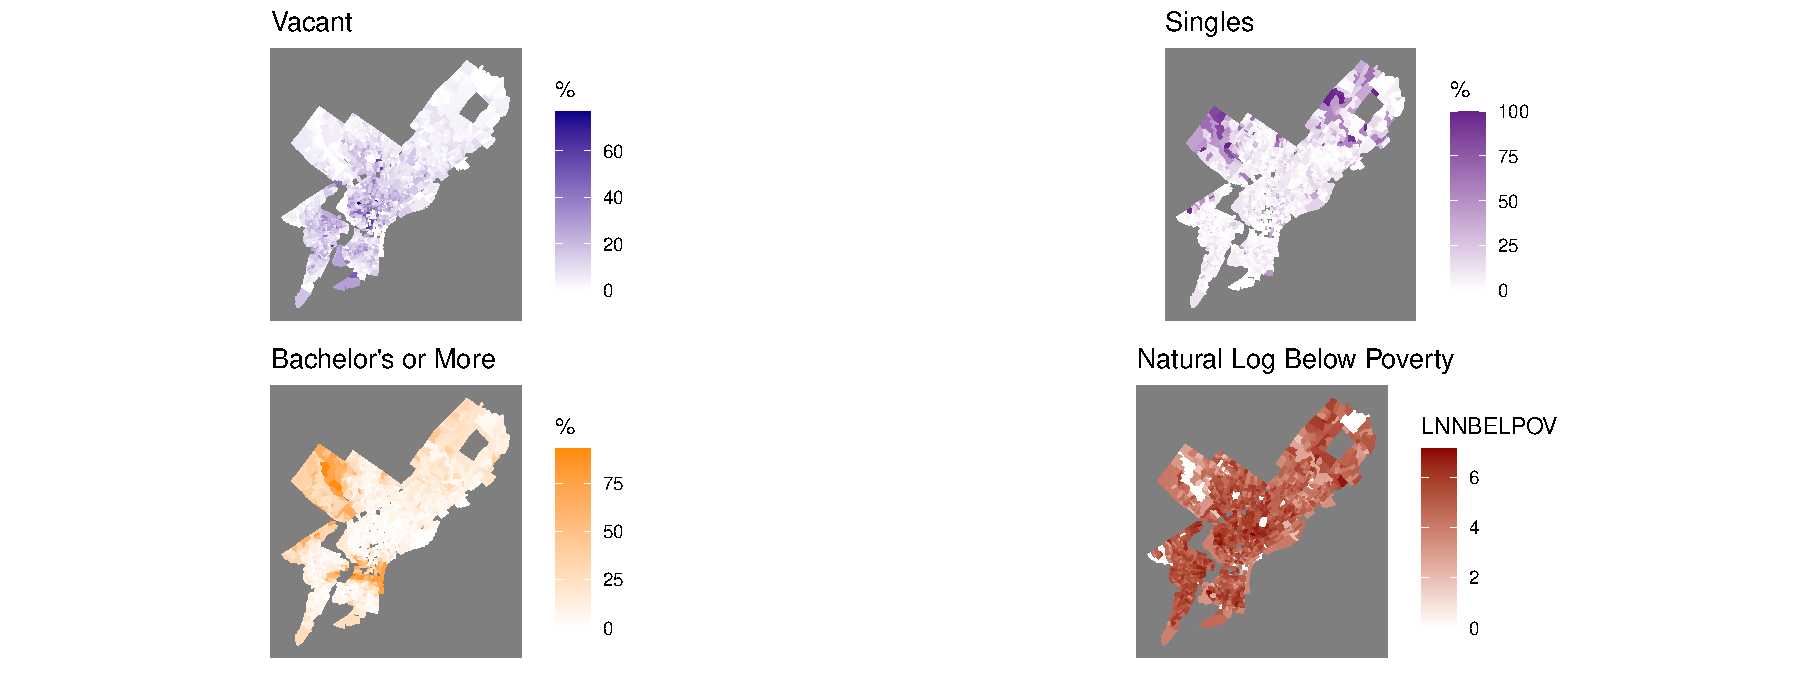
\includegraphics{HW1-Regression_files/figure-latex/variables maps-1.pdf}

\hypertarget{pearson-correlations}{%
\section{Pearson correlations}\label{pearson-correlations}}

\begin{Shaded}
\begin{Highlighting}[]
\NormalTok{predictors }\OtherTok{\textless{}{-}}\NormalTok{ data }\SpecialCharTok{\%\textgreater{}\%}\NormalTok{ dplyr}\SpecialCharTok{::}\FunctionTok{select}\NormalTok{(PCTBACHMOR, PCTVACANT, PCTSINGLES, LNBELPOV100)}

\NormalTok{predictors }\SpecialCharTok{\%\textgreater{}\%} 
  \FunctionTok{correlate}\NormalTok{() }\SpecialCharTok{\%\textgreater{}\%} 
  \FunctionTok{autoplot}\NormalTok{() }\SpecialCharTok{+}
  \FunctionTok{geom\_text}\NormalTok{(}\FunctionTok{aes}\NormalTok{(}\AttributeTok{label =} \FunctionTok{round}\NormalTok{(r,}\AttributeTok{digits=}\DecValTok{2}\NormalTok{)),}\AttributeTok{size =} \DecValTok{8}\NormalTok{)}
\end{Highlighting}
\end{Shaded}

\begin{verbatim}
## Correlation computed with
## * Method: 'pearson'
## * Missing treated using: 'pairwise.complete.obs'
## Registered S3 methods overwritten by 'registry':
##   method               from 
##   print.registry_field proxy
##   print.registry_entry proxy
\end{verbatim}

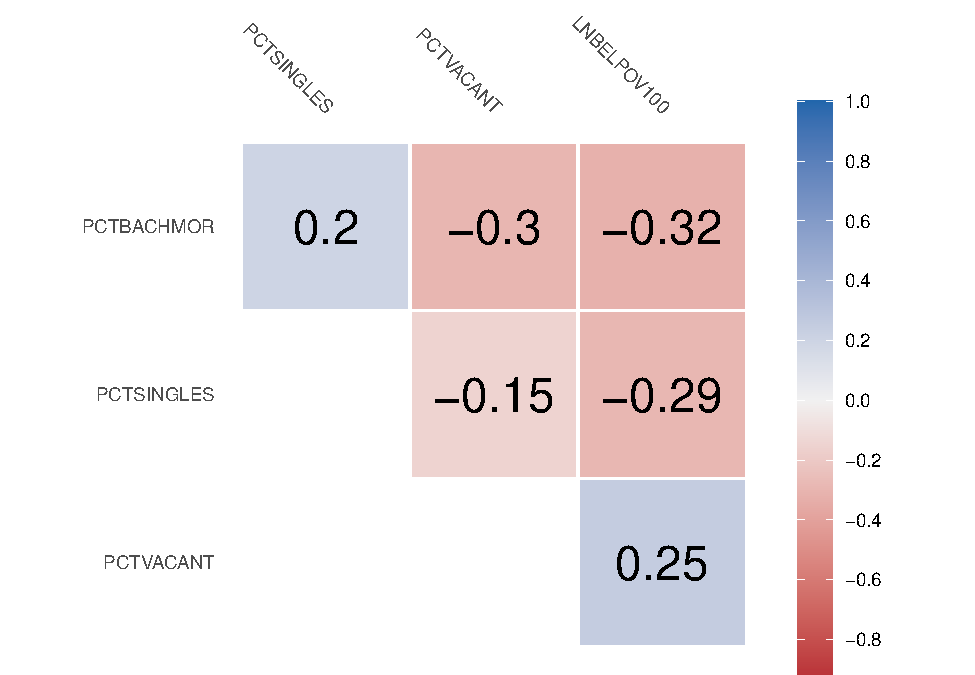
\includegraphics{HW1-Regression_files/figure-latex/pearson-1.pdf}

\hypertarget{regression-analysis}{%
\section{Regression Analysis}\label{regression-analysis}}

\begin{Shaded}
\begin{Highlighting}[]
\DocumentationTok{\#\# Regression Results}

\NormalTok{fit }\OtherTok{\textless{}{-}}\FunctionTok{lm}\NormalTok{(LNMEDHVAL }\SpecialCharTok{\textasciitilde{}}\NormalTok{  PCTVACANT }\SpecialCharTok{+}\NormalTok{ PCTSINGLES }\SpecialCharTok{+}\NormalTok{ PCTBACHMOR }\SpecialCharTok{+}\NormalTok{ LNBELPOV100, }\AttributeTok{data=}\NormalTok{data)}

\FunctionTok{summary}\NormalTok{(fit)}
\end{Highlighting}
\end{Shaded}

\begin{verbatim}
## 
## Call:
## lm(formula = LNMEDHVAL ~ PCTVACANT + PCTSINGLES + PCTBACHMOR + 
##     LNBELPOV100, data = data)
## 
## Residuals:
##      Min       1Q   Median       3Q      Max 
## -2.25825 -0.20391  0.03822  0.21744  2.24347 
## 
## Coefficients:
##               Estimate Std. Error t value             Pr(>|t|)    
## (Intercept) 11.1137661  0.0465330 238.836 < 0.0000000000000002 ***
## PCTVACANT   -0.0191569  0.0009779 -19.590 < 0.0000000000000002 ***
## PCTSINGLES   0.0029769  0.0007032   4.234            0.0000242 ***
## PCTBACHMOR   0.0209098  0.0005432  38.494 < 0.0000000000000002 ***
## LNBELPOV100 -0.0789054  0.0084569  -9.330 < 0.0000000000000002 ***
## ---
## Signif. codes:  0 '***' 0.001 '**' 0.01 '*' 0.05 '.' 0.1 ' ' 1
## 
## Residual standard error: 0.3665 on 1715 degrees of freedom
## Multiple R-squared:  0.6623, Adjusted R-squared:  0.6615 
## F-statistic: 840.9 on 4 and 1715 DF,  p-value: < 0.00000000000000022
\end{verbatim}

\begin{Shaded}
\begin{Highlighting}[]
\FunctionTok{anova}\NormalTok{(fit)}
\end{Highlighting}
\end{Shaded}

\begin{verbatim}
## Analysis of Variance Table
## 
## Response: LNMEDHVAL
##               Df  Sum Sq Mean Sq  F value                Pr(>F)    
## PCTVACANT      1 180.392 180.392 1343.087 < 0.00000000000000022 ***
## PCTSINGLES     1  24.543  24.543  182.734 < 0.00000000000000022 ***
## PCTBACHMOR     1 235.118 235.118 1750.551 < 0.00000000000000022 ***
## LNBELPOV100    1  11.692  11.692   87.054 < 0.00000000000000022 ***
## Residuals   1715 230.344   0.134                                   
## ---
## Signif. codes:  0 '***' 0.001 '**' 0.01 '*' 0.05 '.' 0.1 ' ' 1
\end{verbatim}

\hypertarget{regression-assumptions-checks}{%
\subsection{Regression Assumptions
Checks}\label{regression-assumptions-checks}}

In this section, we will discuss testing model assumptions. We have
already examined the variable distributions in a prior section.

\hypertarget{scatter-plots---linear-relationships-between-variables}{%
\subsubsection{Scatter Plots - Linear Relationships Between
Variables}\label{scatter-plots---linear-relationships-between-variables}}

When running linear regressions, a core assumption is that there is a
linear relationship between the dependent variable and each of the
predictor variables. To check this assumption, we plot the dependent
variable with each of the predictor variables in a scatter plot.

In cases where this assumption is not met, log transformations are often
used. Based on the results of our variable distributions, we have
already conducted log transformations for the dependent variable for
median home value, now LNMEDHVAL, and for the predictor variable for
number of households below poverty, now LNNBELPOV100.

The following scatter plots show the relationship between the dependent
variable, LNMEDHVAL, and each the predictor variables LNNBELPOV100,
PCTBACHMOR, PCTVACANT, and PCTSINGLES. There does not appear to be a
linear relationship between LNMEDHVAL and the predictor variables, even
with log transformations used. The variables all appear heavily skewed -
the relationship between LNNBELPOV and LNBELPOV100 appears to be
negatively skewed, and the individual relationship between the other
three predictors and LNMEDHVAL appears to be heavily positively skewed.

\begin{Shaded}
\begin{Highlighting}[]
\FunctionTok{par}\NormalTok{(}\AttributeTok{mfrow=}\FunctionTok{c}\NormalTok{(}\DecValTok{2}\NormalTok{,}\DecValTok{2}\NormalTok{))}
\FunctionTok{plot}\NormalTok{(data}\SpecialCharTok{$}\NormalTok{LNBELPOV100, data}\SpecialCharTok{$}\NormalTok{LNMEDHVAL)}
\FunctionTok{plot}\NormalTok{(data}\SpecialCharTok{$}\NormalTok{PCTBACHMOR,data}\SpecialCharTok{$}\NormalTok{LNMEDHVAL)}
\FunctionTok{plot}\NormalTok{(data}\SpecialCharTok{$}\NormalTok{PCTVACANT, data}\SpecialCharTok{$}\NormalTok{LNMEDHVAL)}
\FunctionTok{plot}\NormalTok{(data}\SpecialCharTok{$}\NormalTok{PCTSINGLES, data}\SpecialCharTok{$}\NormalTok{LNMEDHVAL)}
\end{Highlighting}
\end{Shaded}

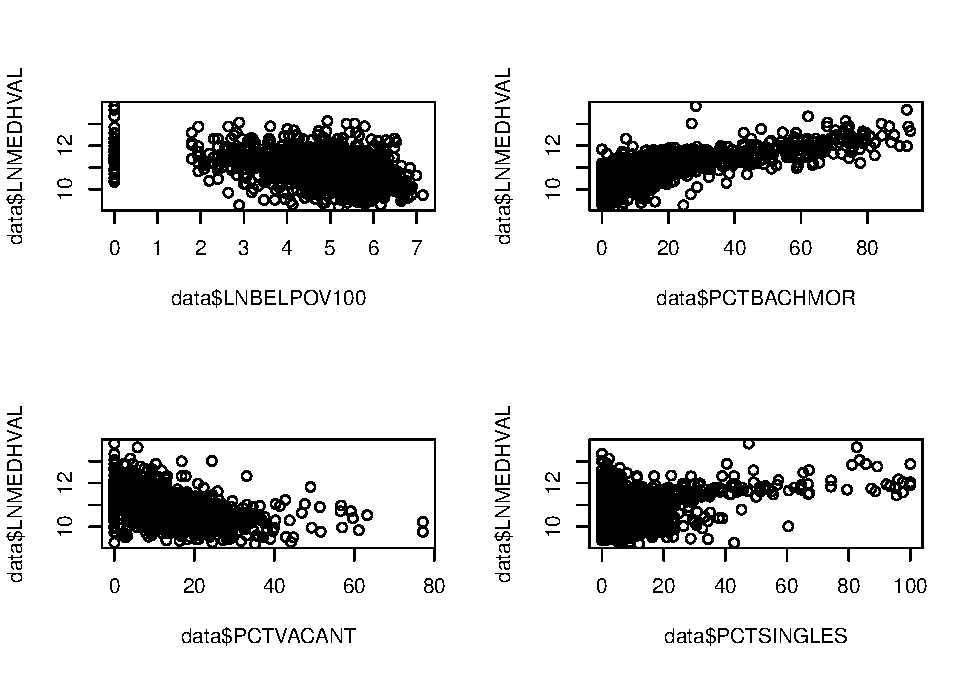
\includegraphics{HW1-Regression_files/figure-latex/scatter-1.pdf}

\#\#\#Histogram of the standardized residuals

Another assumption when running linear regression is that regression
residuals are distributed normally. However, this assumption of
normality is not considered critical in a regression, especially for
data sets with a large number of observations.

In order to compare residuals for different observations, we standardize
the residuals through dividing a residual by its standard error.
Standardizing allows us to observe how many standard deviations a
residual is from our model's estimate

The following histogram of standardized residuals shows that residuals
appear normally distributed.

\begin{Shaded}
\begin{Highlighting}[]
\CommentTok{\#predicted values, residuals and standardized residuals}

\CommentTok{\#Predicted values (y{-}hats)}
\NormalTok{data}\SpecialCharTok{$}\NormalTok{predvals }\OtherTok{\textless{}{-}} \FunctionTok{fitted}\NormalTok{(fit) }
\CommentTok{\#Residuals}
\NormalTok{data}\SpecialCharTok{$}\NormalTok{resids }\OtherTok{\textless{}{-}} \FunctionTok{residuals}\NormalTok{(fit)}
\CommentTok{\#Standardized Residuals}
\NormalTok{data}\SpecialCharTok{$}\NormalTok{stdres }\OtherTok{\textless{}{-}} \FunctionTok{rstandard}\NormalTok{(fit)}

\FunctionTok{hist}\NormalTok{(data}\SpecialCharTok{$}\NormalTok{stdres, }\AttributeTok{breaks=}\DecValTok{100}\NormalTok{)}
\end{Highlighting}
\end{Shaded}

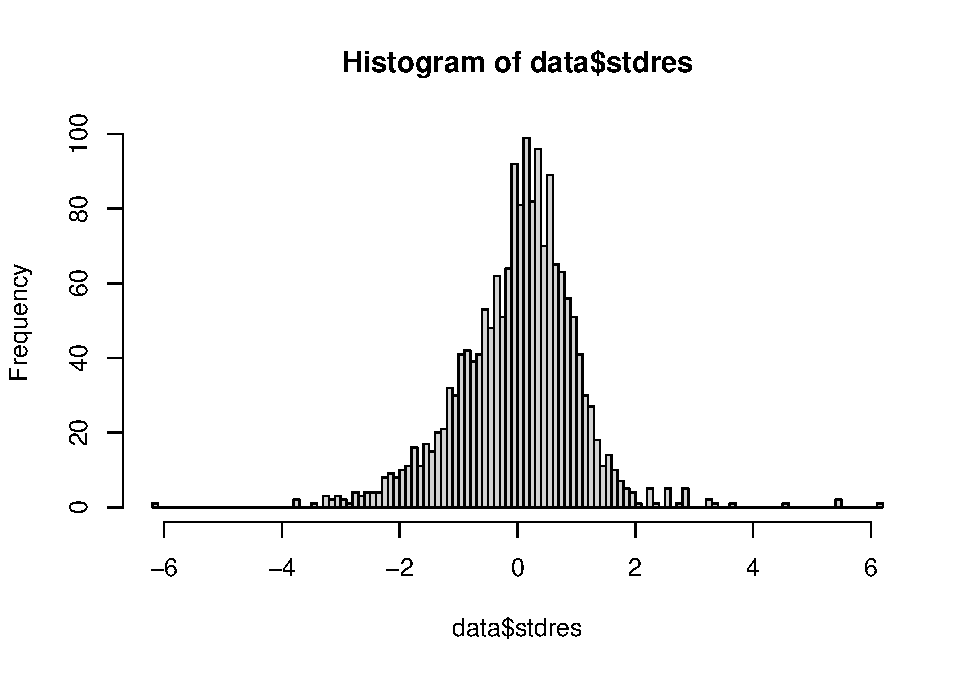
\includegraphics{HW1-Regression_files/figure-latex/resid plot-1.pdf}

\#\#\#Scatter Plot - Standardized Residual by Predicted Value

An additional core assumption of linear regression is that there is
constant variance in residuals compared to the predicted values of the
model - this relationship is referred to as homoscedastic. If
non-constant variance is observed, the relationship is heteroscedastic.

Given that there multiple predictors, we can plot the standardized
residuals of the model by our predicted values of LNMEDHVAL. The scatter
plot of standardized residuals appears to show a slight heteroscedastic
relationship, based on a small ``bow-tie'' shape present around the
predicted value of 11.5.

Outliers also appear to be present based on our scatter plot - there are
several positive standardized residuals above 4 standard deviations
above 0 and at least one standardized residual beyond -6 standard
deviation below 0.

The standardized residuals also appear to be heavily clustered around
between the predicted values of about 10.5 to 11.5.

\begin{Shaded}
\begin{Highlighting}[]
\FunctionTok{plot}\NormalTok{(data}\SpecialCharTok{$}\NormalTok{predvals, data}\SpecialCharTok{$}\NormalTok{stdres, }\AttributeTok{xlab =} \StringTok{"Predicted Values "}\NormalTok{, }\AttributeTok{ylab =} \StringTok{"Standardized Residuals "}\NormalTok{, }\AttributeTok{main =} \StringTok{"Predicted Values vs. Standardized Residuals "}\NormalTok{)}
\end{Highlighting}
\end{Shaded}

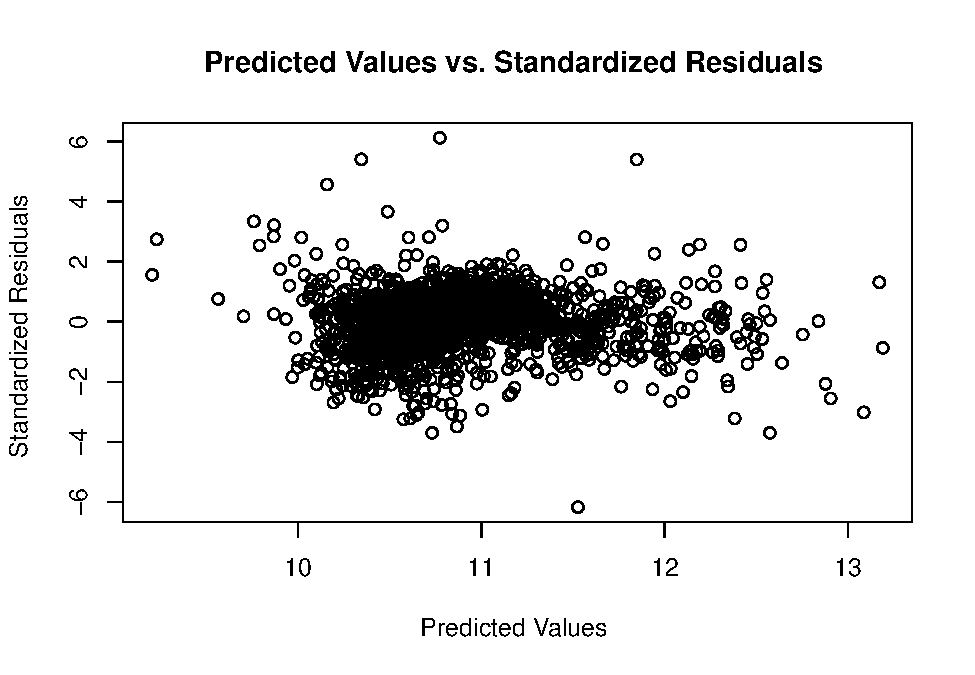
\includegraphics{HW1-Regression_files/figure-latex/plot_stand_resid-1.pdf}
\#\#\#Spatial Autocorrelation of Variables

Based on the maps of the dependent variable LNMEDHVAL and the predictor
variables, we can estimate whether observations of each variable appear
to show spatial autocorrelation - defined as observing the degree to
which similar values cluster near each other. Our variables may appear
to spatial autocorrelation

\#\#\#Choropleth map of the standardized regression residuals

\begin{Shaded}
\begin{Highlighting}[]
\NormalTok{map2 }\OtherTok{\textless{}{-}} \FunctionTok{cbind}\NormalTok{(map, data }\SpecialCharTok{\%\textgreater{}\%}\NormalTok{ dplyr}\SpecialCharTok{::}\FunctionTok{select}\NormalTok{(stdres))}

\FunctionTok{ggplot}\NormalTok{()}\SpecialCharTok{+}
  \FunctionTok{geom\_sf}\NormalTok{(}\AttributeTok{data=}\NormalTok{map2, }\FunctionTok{aes}\NormalTok{(}\AttributeTok{fill =}\NormalTok{ stdres), }\AttributeTok{color =} \ConstantTok{NA}\NormalTok{)}\SpecialCharTok{+}
  \FunctionTok{scale\_fill\_viridis\_c}\NormalTok{()}\SpecialCharTok{+}
  \FunctionTok{labs}\NormalTok{(}\AttributeTok{title =} \StringTok{"Standardized Regression Residuals"}\NormalTok{) }\SpecialCharTok{+}
  \FunctionTok{theme\_dark}\NormalTok{() }\SpecialCharTok{+}
  \FunctionTok{theme}\NormalTok{( }
    \AttributeTok{panel.grid.major =} \FunctionTok{element\_blank}\NormalTok{(),}
    \AttributeTok{panel.grid.minor =} \FunctionTok{element\_blank}\NormalTok{(),}
    \AttributeTok{axis.ticks =} \FunctionTok{element\_blank}\NormalTok{(),}
    \AttributeTok{axis.text =} \FunctionTok{element\_blank}\NormalTok{()}
\NormalTok{    )}
\end{Highlighting}
\end{Shaded}

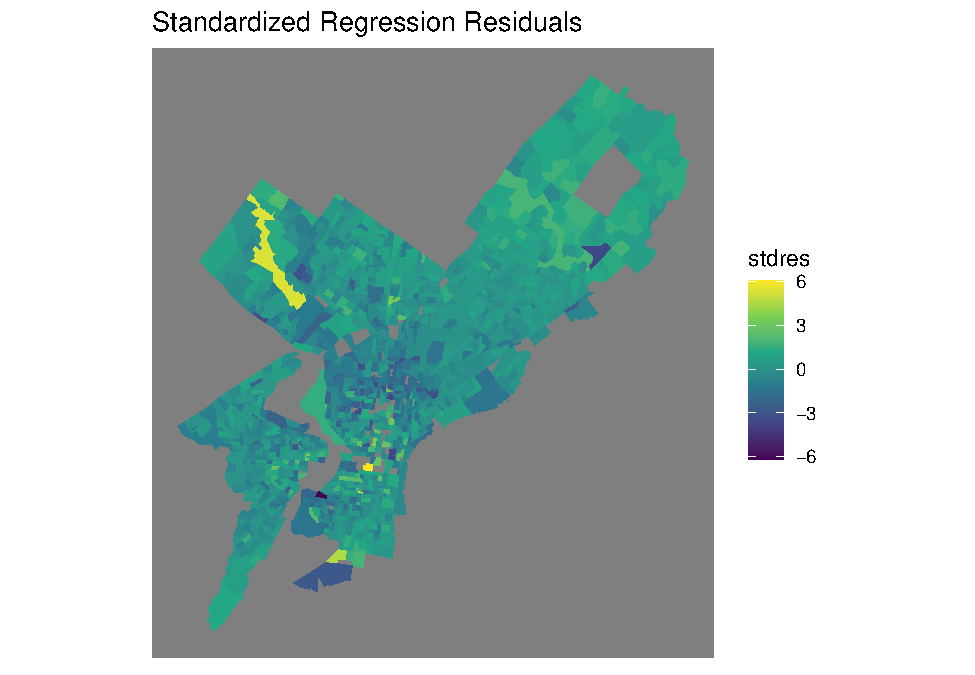
\includegraphics{HW1-Regression_files/figure-latex/resid map-1.pdf}

\hypertarget{additional-models}{%
\subsection{Additional Models}\label{additional-models}}

\#\#\#Stepwise Regression

\begin{Shaded}
\begin{Highlighting}[]
\NormalTok{step }\OtherTok{\textless{}{-}} \FunctionTok{stepAIC}\NormalTok{(fit, }\AttributeTok{direction=}\StringTok{"both"}\NormalTok{)}
\end{Highlighting}
\end{Shaded}

\begin{verbatim}
## Start:  AIC=-3448.07
## LNMEDHVAL ~ PCTVACANT + PCTSINGLES + PCTBACHMOR + LNBELPOV100
## 
##               Df Sum of Sq    RSS     AIC
## <none>                     230.34 -3448.1
## - PCTSINGLES   1     2.407 232.75 -3432.2
## - LNBELPOV100  1    11.692 242.04 -3364.9
## - PCTVACANT    1    51.546 281.89 -3102.7
## - PCTBACHMOR   1   199.020 429.36 -2379.0
\end{verbatim}

\begin{Shaded}
\begin{Highlighting}[]
\CommentTok{\# display results}
\NormalTok{step}\SpecialCharTok{$}\NormalTok{anova}
\end{Highlighting}
\end{Shaded}

\begin{verbatim}
## Stepwise Model Path 
## Analysis of Deviance Table
## 
## Initial Model:
## LNMEDHVAL ~ PCTVACANT + PCTSINGLES + PCTBACHMOR + LNBELPOV100
## 
## Final Model:
## LNMEDHVAL ~ PCTVACANT + PCTSINGLES + PCTBACHMOR + LNBELPOV100
## 
## 
##   Step Df Deviance Resid. Df Resid. Dev       AIC
## 1                       1715   230.3435 -3448.073
\end{verbatim}

\#\#\#Cross-Validation

\begin{Shaded}
\begin{Highlighting}[]
\NormalTok{fit1 }\OtherTok{\textless{}{-}} \FunctionTok{lm}\NormalTok{(LNMEDHVAL }\SpecialCharTok{\textasciitilde{}}\NormalTok{ PCTVACANT }\SpecialCharTok{+}\NormalTok{ PCTSINGLES }\SpecialCharTok{+}\NormalTok{ PCTBACHMOR }\SpecialCharTok{+}\NormalTok{ LNBELPOV100, }\AttributeTok{data=}\NormalTok{data)}
\NormalTok{cv1 }\OtherTok{\textless{}{-}} \FunctionTok{CVlm}\NormalTok{(}\AttributeTok{data=}\NormalTok{data, fit1, }\AttributeTok{m=}\DecValTok{5}\NormalTok{)}
\end{Highlighting}
\end{Shaded}

\begin{verbatim}
## Warning in CVlm(data = data, fit1, m = 5): 
## 
##  As there is >1 explanatory variable, cross-validation
##  predicted values for a fold are not a linear function
##  of corresponding overall predicted values.  Lines that
##  are shown for the different folds are approximate
\end{verbatim}

\begin{Shaded}
\begin{Highlighting}[]
\NormalTok{mse1 }\OtherTok{\textless{}{-}} \FunctionTok{attr}\NormalTok{(cv1, }\StringTok{"ms"}\NormalTok{)}
\NormalTok{rmse1 }\OtherTok{\textless{}{-}} \FunctionTok{sqrt}\NormalTok{(mse1)                       }\CommentTok{\#Obtaining RMSE for model 1}
\NormalTok{rmse1}

\NormalTok{fit2 }\OtherTok{\textless{}{-}} \FunctionTok{lm}\NormalTok{(LNMEDHVAL }\SpecialCharTok{\textasciitilde{}}\NormalTok{ PCTVACANT }\SpecialCharTok{+}\NormalTok{ MEDHHINC, }\AttributeTok{data=}\NormalTok{data)}
\NormalTok{cv2 }\OtherTok{\textless{}{-}} \FunctionTok{CVlm}\NormalTok{(}\AttributeTok{data=}\NormalTok{data, fit2, }\AttributeTok{m=}\DecValTok{5}\NormalTok{)}
\end{Highlighting}
\end{Shaded}

\begin{verbatim}
## Warning in CVlm(data = data, fit2, m = 5): 
## 
##  As there is >1 explanatory variable, cross-validation
##  predicted values for a fold are not a linear function
##  of corresponding overall predicted values.  Lines that
##  are shown for the different folds are approximate
\end{verbatim}

\begin{Shaded}
\begin{Highlighting}[]
\NormalTok{mse2 }\OtherTok{\textless{}{-}} \FunctionTok{attr}\NormalTok{(cv2, }\StringTok{"ms"}\NormalTok{)}
\NormalTok{rmse2 }\OtherTok{\textless{}{-}} \FunctionTok{sqrt}\NormalTok{(mse2)                       }\CommentTok{\#Obtaining RMSE for model 2}
\NormalTok{rmse2}

\NormalTok{rmse\_both }\OtherTok{\textless{}{-}} \FunctionTok{cbind}\NormalTok{(rmse1, rmse2)}

\NormalTok{rmse\_both }\SpecialCharTok{\%\textgreater{}\%} \FunctionTok{kbl}\NormalTok{() }\SpecialCharTok{\%\textgreater{}\%} \FunctionTok{kable\_minimal}\NormalTok{(}\AttributeTok{full\_width =} \ConstantTok{FALSE}\NormalTok{)}
\end{Highlighting}
\end{Shaded}

\hypertarget{additional-models-1}{%
\subsection{Additional Models}\label{additional-models-1}}

\hypertarget{discussion-and-limitations}{%
\section{Discussion and Limitations}\label{discussion-and-limitations}}

\end{document}
